%
% Copyright (c) 2017  Zubax Robotics OU  <info@zubax.com>
%
% Distributed under BY-NC-ND (attribution required, non-commercial use only, no derivatives).
%

\documentclass{zubaxdoc}
\graphicspath{{document_templates/documentation_template_latex/}}

\usepackage{ConfigParamIndex}
\usepackage{makecell}

\title{Zubax GNSS 2 Datasheet}

\begin{document}
\frontmatter

\begin{titlepage}

\section*{Overview}

Zubax GNSS 2 is a multipurpose high-performance positioning module interfaced via CAN bus, USB, and UART.
It includes a state-of-the-art multi-system GPS/\allowbreak{}GLONASS receiver,
a high-precision barometric altimeter, and a 3-axis compass with thermal compensation.

\section*{Features}

\begin{itemize}
    \item State-of-the-art concurrent GPS/GLONASS receiver u-blox MAX-M8Q.
    \begin{itemize}
    	\item Full RF shielding of the GNSS circuits ensures reliable operation in high-EMI environments.
    	\item 35 mm high-gain patch antenna with large ground plane for reliable reception even in deep urban canyons.
    	\item Analog front-end with LNA and SAW ensures high noise resilience.
    	\item Supercapacitor-based backup power source enables low time-to-first-fix (a few seconds).
    	\item Up to 15 Hz update rate.
    \end{itemize}
	\item High precision digital barometer TE Connectivity MS5611.
    \item High precision 3-axis digital compass STMicroelectronics LIS3MDL with thermal compensation.
	\item Supported interfaces:
    \begin{itemize}
        \item CAN, with optional double redundancy.
        \item UART.
        \item USB port, no drivers needed.
    \end{itemize}
    \item High quality assurance:
    \begin{itemize}
        \item Every manufactured unit undergoes a strict testing procedure.
        The testing log for each produced unit is available to the user via the website at\\
        \url{https://device.zubax.com/device_info}.
        \item Protection against unlicensed (counterfeit) production by means of a digital signature
        installed on every manufactured unit.
    \end{itemize}
\end{itemize}

\BeginRightColumn

\section*{Applications}

\begin{itemize}
	\item Positioning module for unmanned vehicles (aerial, ground, underwater, etc) and robots.
    \item General-purpose embedded positioning module.
\end{itemize}

\centering
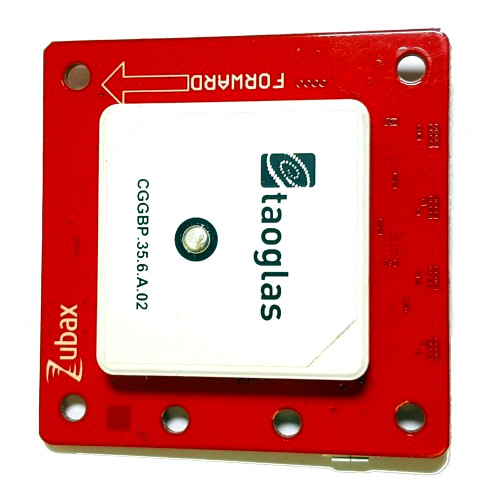
\includegraphics[width=0.45\textwidth]{GNSS_top}
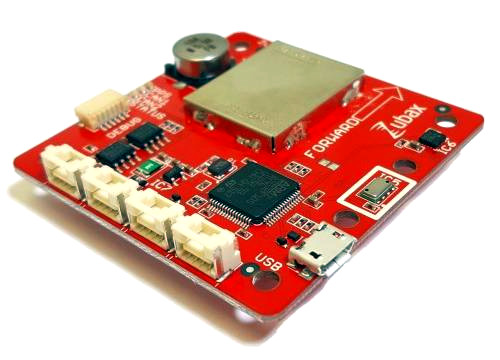
\includegraphics[width=0.45\textwidth]{GNSS_bottom}
\end{titlepage}

\tableofcontents
\clearpage
\listoffigures
\BeginRightColumn
\listoftables

\mainmatter

\chapter{Overview}

Zubax GNSS 2 is a multipurpose high-performance positioning module interfaced via CAN bus, USB, and UART.
It includes a state-of-the-art multi-system GPS/GLONASS receiver, a high-precision barometric altimeter, and a 3-axis compass with thermal compensation.
Zubax GNSS 2 supports a variety of standard protocols, which ensures compatibility with third party software and hardware: UAVCAN (over CAN bus), NMEA 0183 (over USB and UART), and the u-Blox M8 binary protocol.

\section{Sensor suite}

\subsection{GNSS receiver}

The device employs the \textbf{u-Blox MAX-M8Q} GNSS receiver module.
Please refer to the specifications provided by u-Blox to gain additional information about the module.

\subsection{Digital barometric altimeter}

The device employs the \textbf{TE Connectivity MS5611} digital barometric altimeter.
Please refer to the specifications provided by TE Connectivity to gain additional information about the sensor.

\subsection{Three-axis digital compass with thermal compensation}

The device employs the \textbf{STMicroelectronics LIS3MDL} digital three-axis compass with thermal compensation.
Please refer to the specifications provided by STMicroelectronics to gain additional information about the sensor.

Zubax GNSS v2.1 and older (manufacturing years 2015--2016) used to employ \textbf{Honeywell HMC5983} instead.
These modifications of the hardware are no longer manufactured.

\section{Accessories}

Zubax GNSS 2 can be used with the following accessories:

\begin{itemize}
    \item Plastic enclosure described in the section \ref{sec:enclosure}.
    \item UAVCAN cabling and related items. Refer to \url{https://kb.zubax.com/x/EoAh} for more information.
    \item Zubax Dronecode probe. Refer to \url{https://kb.zubax.com/x/iIAh} for more information.
\end{itemize}

Please contact your supplier for ordering information.

\subsection{Enclosure}\label{sec:enclosure}

Zubax GNSS 2 is intended for integration into the end system in the form of the bare PCB,
as this facilitates lower weight and tighter arrangement of components
in the end device, all of which are desirable properties in the target application domains.

Shall it be desired to provide additional mechanical protection for the device or to install it away from possible sources of electromagnetic interference, the plastic components pictured on the figure \ref{enclosure} can be used.
Please contact your supplier for the ordering information;
alternatively, visit \url{https://github.com/Zubax/zubax_gnss} to download
the 3D printable models suitable for in-house manufacturing.

\begin{figure}[hbt]
	\centering
	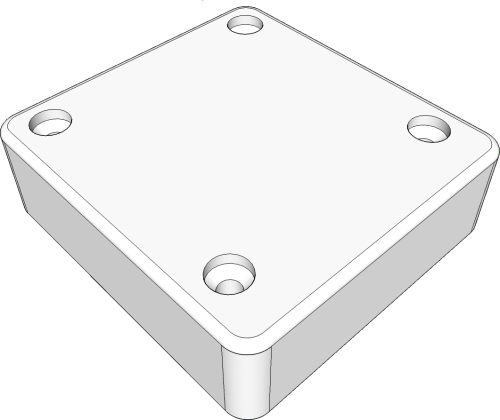
\includegraphics[width=0.45\textwidth]{enclosure_assembled_top}
	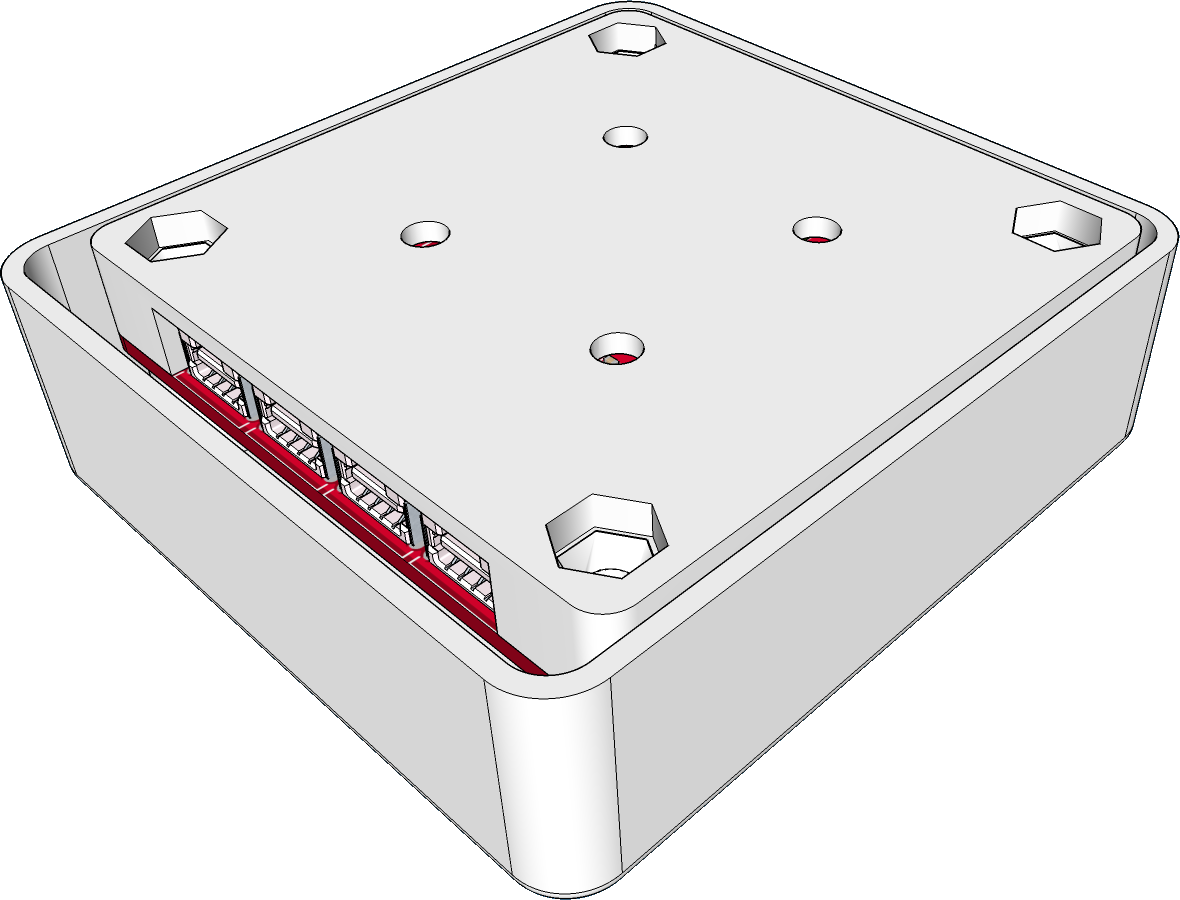
\includegraphics[width=0.45\textwidth]{enclosure_assembled_bottom}
	\caption{Plastic enclosure suitable for 3D-printing, top and bottom, assembled.\label{enclosure}}
\end{figure}

\begin{figure}[hbt]
	\centering
	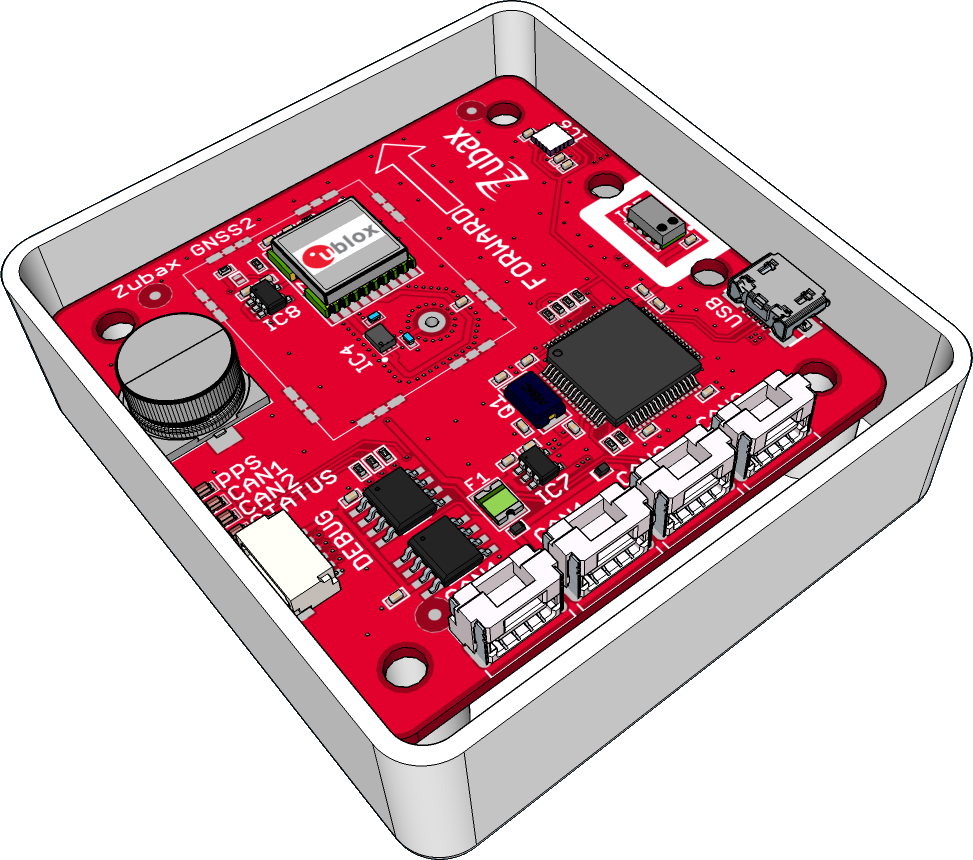
\includegraphics[width=0.45\textwidth]{enclosure_pcb_top}
	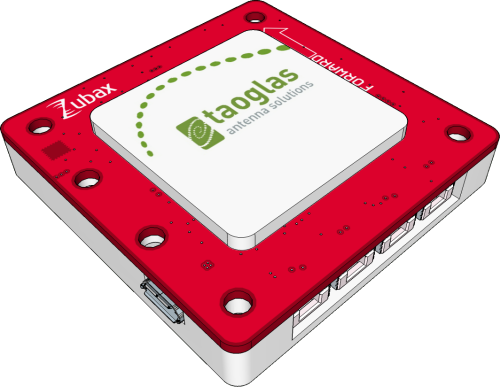
\includegraphics[width=0.45\textwidth]{enclosure_pcb_bottom}
	\caption{Top and bottom parts of the enclosure with the device inside.}
\end{figure}

\section{Quality assurance}

Every manufactured Zubax GNSS 2 undergoes an automated testing procedure that validates that
the device is functioning as designed.
The test log for every manufactured device is available on the web at
\url{https://device.zubax.com/device_info}.
This feature can be used to facilitate traceability of purchased devices and
provide additional safety assurances.

Besides testing, every manufactured device has a digital signature installed,
that can be used as a strong protection against unlicensed or counterfeit manufacturing.
Please contact Zubax Robotics
to find out the specifics about digital signature verification.

\chapter{Characteristics}

\section{Absolute maximum ratings}

Subjecting the device to stresses beyond those specified in this section may cause
permanent damage to the device.
Proper operation of the device within the ranges specified in this section is not implied.

\begin{ZubaxSimpleTable}{Absolute maximum ratings}{|c X|c c|c|}
    Symbol            & Parameter                & Min  & Max & Unit \\
	$V_\text{supply}$ & Supply voltage           & -0.3 & 6   & V \\
	$T_\text{oper}$   & Operating temperature    & -40  & 105 & \degree{}C \\
	                  & UART input voltage 		& -0.3 & 6   & V\\
	                  & CAN H/L input voltage    & -4   & 16  & V\\
\end{ZubaxSimpleTable}

\section{Environmental conditions}\label{environmental_conditions}

The GNSS hot start feature is not expected to work reliably below -20\degree{}C
due to poor performance of the supercapacitor-based backup power source at low temperatures.
However, this should not have any adverse side effects on the general performance of
the unit except that the time-to-first-fix (TTFF) may be higher than normal.

Magnetic fields whose magnitude exceeds the limit may render the compass temporarily dysfunctional.
Other components are unlikely to be affected.

\begin{ZubaxTableWrapper}{Environmental conditions}
    \begin{ZubaxWrappedTable}{|c X|l c|c|c|}
        Symbol            & Parameter                     &  Min & Max & Unit \\
        $T_\text{oper}$   & Operating temperature         & -40  & 100 & \degree{}C \\
        $B$               & Magnetic field strength       &      & 9   & Gauss \\
        $\phi_\text{oper}$& Operating humidity\tnote{1}   & 0    & 100 & \%RH\\
        $h_\text{oper}$   & Operating altitude above mean sea level (MSL) &     & 10  & km\\
    \end{ZubaxWrappedTable}
    \begin{tablenotes}
        \item[1] Condensation not permitted.
    \end{tablenotes}
\end{ZubaxTableWrapper}

\section{Reliability}

Please contact Zubax Robotics for additional reliability and safety information.

\begin{ZubaxSimpleTable}{Reliability}{|c X|c|c|}
    Symbol & Parameter & Typ & Unit \\
	MTTF   & Mean time to failure & 500000 & hours \\
\end{ZubaxSimpleTable}

\section{Communication interfaces}

Zubax GNSS 2 features three communication interfaces. Each is described in detail in the subsequent parts of this document.
\begin {itemize}
\item Doubly redundant UAVCAN interface with two connectors for each interface.
\item USB port.
\item Dronecode port.
\end{itemize}

\subsection{CAN bus interface}

This interface provides full access to all features of Zubax GNSS 2, including the output of measurements,
reconfiguration, time synchronization, firmware update, etc.

The connector type is UAVCAN Micro connector (JST GH)\footnote{\url{https://kb.zubax.com/x/EoAh}}.

\begin{ZubaxTableWrapper}{Characteristics of CAN bus interfaces}
	\begin{ZubaxWrappedTable}{|c X|c c c|c|}
		Symbol  & Parameter                                 & Min  & Typ  & Max  & Unit \\
		        & Bit rate                                  & 20   &      & 1000 & Kbps \\
		        & Positive-going input threshold voltage    &      & 750  & 900  & mV \\
		        & Negative-going input threshold voltage    & 500  & 600  &      & mV \\
		        & Differential output voltage, dominant     & 1.5  & 2.0  & 3.0  & V \\
		        & Differential output voltage, recessive    & -120 & 0    & 12   & mV \\
		        & Inter-connector current\tnote{1}          & -1   &      & 1    & A \\
		        & Connector resistance during device lifetime &    & 30   & 50   & $\text{m}\Omega$ \\
	\end{ZubaxWrappedTable}
	\begin{tablenotes}
	    \item [1] The limit is imposed by the PCB.
	\end{tablenotes}
\end{ZubaxTableWrapper}

\subsection{USB interface}

The device implements a full-speed USB 2.0 port with the standard CDC ACM interface.
The device features driverless compatibility with all major operating systems (Windows, GNU/Linux, Mac).

This interface can be used for NMEA output, configuration, firmware update,
and general-purpose CLI\footnote{Command line interface.} access.

The connector type is USB micro B (which is the most common USB connector type).

Note that the virtual serial port interface is sensitive to the baud rate configuration.
More details are provided in the section \ref{usb_protocol_selection}.

\subsection{Dronecode debug port interface}

The device features a Dronecode debug port interface available via the standard
Dronecode Debug Mini connector (DCD-Mini)\footnote{\url{https://wiki.dronecode.org/workgroup/connectors/start}}.

\begin{ZubaxSimpleTable}{Dronecode debug port characteristics}{|c X|c c c|c|}
	Symbol  & Parameter                                 & Min  & Typ  & Max  & Unit \\
			& Low-level input voltage                   & -0.3 & 0    & 1.6  & V\\
			& High-level input voltage                  & 2.1  & 3.3  & 5.5  & V\\
			& Low-level output voltage                  & 0    & 0    & 0.5  & V\\
			& High-level output voltage                 & 2.8  & 3.3  & 3.4  & V\\
			& Source/sink current via data pins         &      &      & 10   & mA\\
			& UART RX pull down resistance              & 30   & 40   & 50   & $\text{k}\Omega$\\
	        & Connector resistance during device lifetime &    & 20   & 40   & $\text{m}\Omega$\\
\end{ZubaxSimpleTable}

\section{Power supply}

The device can be powered via the following inputs:
\begin {itemize}
\item Any single UAVCAN port.
\item Both UAVCAN ports simultaneously
(the power supply circuit prevents direct current flow between these power inputs).
\item USB port.
\item Dronecode port (hardware revisions v2.1 and newer).
\end{itemize}

It is allowed to power the device simultaneously via USB and UAVCAN, since the power supply circuits prevent back-powering via these interfaces.
It is not recommended to supply power via the Dronecode port while any other power input is used concurrently.

The power supply characteristics documented in the following table are invariant to the power input used.

\begin{ZubaxSimpleTable}{Power supply}{|c X|c c c|c|X|}
     Symbol             & Parameter      & Min & Typical & Max & Unit & Note \\
	 $V_\text{supply}$  & Supply voltage & 4.0 & 5.0     & 5.5 & V    & Any power input\\
	 $I_\text{supply}$  & Supply current & 70  & 95      & 180 & mA   & Any power input\\
\end{ZubaxSimpleTable}

\chapter{Continuous self-diagnostics}\label{sec:self-diagnostics}

Zubax GNSS 2 continuously monitors its own status and sensor outputs for anomalies and malfunctions.
Results of the continuous self-testing are mapped to three health codes: OK, Warning, and Error.
The table below documents how the device uses health codes to report its status.

\begin{ZubaxSimpleTable}{Self-diagnostic health codes}{|l|X|}
    Health        & Conditions    \\
    OK            & Everything is OK; all enabled sensors are functioning properly.\\
    Warning       & See below. \\
    Error         & Sensor malfunction.
                    The device may stop sending the measurements obtained from the failed sensor. \\
\end{ZubaxSimpleTable}

Possible reasons for the health being Warning:

\begin{itemize}
    \item GNSS fix quality is below the configured threshold (section \ref{sec:configuration_parameters})
    (disabled by default).
    \item Determined environmental conditions exceed the specified safe limits
    (section \ref{environmental_conditions}).
    \item Magnetic field strength vector remained zero for several seconds (likely a sensor malfunction).
\end{itemize}

\chapter{LED Indication}

The physical locations of the LED indicators are documented in the chapter \ref{sec:mechanical}.

\section{PPS LED indicator}

This LED indicator blinks with the rate of 1 Hz if the GNSS receiver has a navigation fix.

\section{Status LED indicator}

This LED indicator shows the health of the device derived from the continuous self-diagnostics as described
in the chapter \ref{sec:self-diagnostics}.

\newcommand{\LEDX}{{\rule{0.4em}{0.8em}}}
\newcommand{\LEDO}{{\rule{0.4em}{0.1em}}}

\begin{ZubaxSimpleTable}{Status LED indication}{|X|X|X|}
Health 	& Blinking pattern & On/Off duration [second] \\
OK      & \LEDX\LEDO\LEDO\LEDO\LEDO\LEDO\LEDO\LEDO\LEDO\LEDO\LEDO\LEDO\LEDO\LEDO\LEDO\LEDO\LEDO\LEDO\LEDO\LEDO
        & 0.05/0.95 seconds \\
Warning & \LEDX\LEDO\LEDO\LEDO\LEDO\LEDX\LEDO\LEDO\LEDO\LEDO\LEDX\LEDO\LEDO\LEDO\LEDO\LEDX\LEDO\LEDO\LEDO\LEDO
        & 0.05/0.25 seconds \\
Error   & \LEDX\LEDO\LEDX\LEDO\LEDX\LEDO\LEDX\LEDO\LEDX\LEDO\LEDX\LEDO\LEDX\LEDO\LEDX\LEDO\LEDX\LEDO\LEDX\LEDO
        & 0.05/0.05 seconds \\
\end{ZubaxSimpleTable}

\section{CAN1 and CAN2 LED indicators}

These LED indicators display the intensity of the CAN bus traffic per interface.

Each blink indicates that a CAN frame was successfully transmitted or successfully received during
the last few milliseconds.
Under a high bus load, these LED indicators are expected to glow steadily.
If an interface is not connected to the bus, the corresponding LED indicator will be inactive (turned off),
even if the device is actually attempting to transmit.

Note that the CAN traffic filtered out by the hardware acceptance filters of the device will not affect the
state of the LED indicators.

\section{LED indication during firmware update and bootup}

\subsection{Hardware version 2.2 and newer}

This section is valid for all hardware manufactured since 2017.

During the first few seconds after power-on or after restart, and also in the process of firmware update, Zubax GNSS 2 uses its LED indicators in a different way, as described in the chapter \ref{sec:bootloader}.

\subsection{Hardware version 2.0 and 2.1}

This section is valid for the hardware manufactured until 2016, inclusive.

During the first few seconds after power-on or after restart, and also in the process of firmware update, Zubax GNSS 2 uses its LED indicators in a different way, as described in the table below.

\begin{ZubaxSimpleTable}{LED indication at bootup for hardware v2.0 and 2.1}{| X | c | c | c|}
Status & INFO & CAN1 & CAN2 \\
CAN bit rate detection &  & Solid & \\
Dynamic node ID allocation & Solid & &  \\
Update in progress & Solid & Solid & \\
\end{ZubaxSimpleTable}

\chapter{UAVCAN interface}

For the background information about the UAVCAN interface please refer to the Zubax Knowledge Base
at \url{https://kb.zubax.com/x/F4Ah} and the official UAVCAN website at \url{http://uavcan.org}.

The UAVCAN interface enables access to all features of Zubax GNSS 2.
This interface provides access to the GNSS solutions, magnetic field and barometric pressure measurements,
precise time (via the time synchronization master), device configuration parameters, firmware upgrade feature,
and so on.

This section documents the UAVCAN interface that is available during the normal operation of the device,
omitting the logic specific to the firmware update mode, which is documented separately in the chapter
\ref{sec:bootloader}.

\section{Device interconnection}

Zubax GNSS 2 can be used with doubly-redundant and non-redundant CAN buses.
In the latter case, only CAN1 can be used, and CAN2 must be left unconnected.
The figure \ref{can_daisy_chain} shows the possible device interconnection schemes.

\begin{figure}[hbt]
    \center
	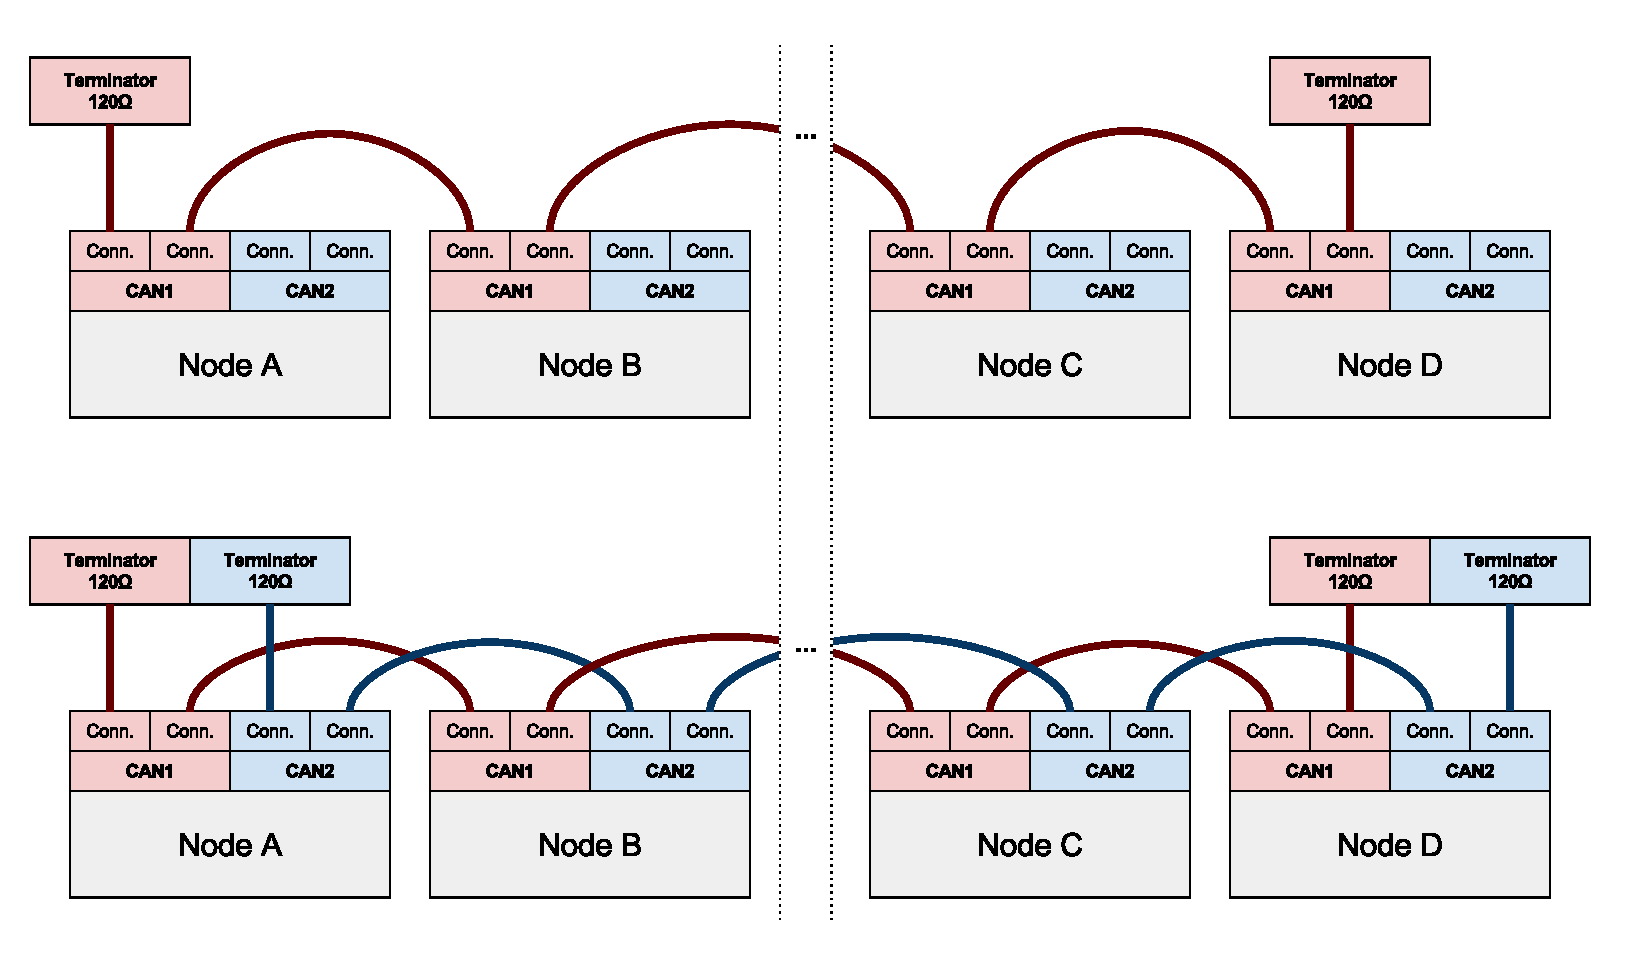
\includegraphics[width=1\textwidth]{can_daisy_chain}
	\caption{CAN bus interconnection diagram for non-redundant and a doubly-redundant interfaces.
	\label{can_daisy_chain}}
\end{figure}

\section{Basic functions}

\subsection{Node status reporting}

The standard node status message \verb|uavcan.protocol.NodeStatus| is broadcasted at 1 hertz.
The node health codes are mapped directly to the output of the self-diagnostic feature
documented in the chapter \ref{sec:self-diagnostics}.
The operating mode codes are summarized below.

\begin{ZubaxSimpleTable}{UAVCAN node mode code interpretation}{|l|X|}
Node mode & Meaning  \\
OPERATIONAL        & Operating normally. \\
INITIALIZATION     & The firmware has just started and is not ready to begin normal operation yet. \\
MAINTENANCE        & See the chapter \ref{sec:bootloader} about the bootloader. \\
SOFTWARE\_{}UPDATE & See the chapter \ref{sec:bootloader} about the bootloader. \\
OFFLINE            & Not applicable. \\
\end{ZubaxSimpleTable}

The vendor-specific status code field is not used by the device.

Node uptime is reported from the moment when the firmware is started.
The time while the bootloader was running is not included in the reported uptime value.

\subsection{Node identification}\label{sec:uavcan_node_identification}

The service \verb|uavcan.protocol.GetNodeInfo| is responded to as follows.

All fields of the nested structure \verb|uavcan.protocol.SoftwareVersion|
are populated, which are \verb|major|, \verb|minor|, \verb|vcs_commit|, and \verb|image_crc|.

The following fields of the nested structure \verb|uavcan.protocol.HardwareVersion|
are always populated: \verb|major|, \verb|minor|, \verb|unique_id|, and \verb|certificate_of_authenticity|.

The field \verb|name| is set to the string \verb|com.zubax.gnss|.

\subsection{Node restarting}

The service \verb|uavcan.protocol.RestartNode|, if the provided magic number is correct,
unconditionally reboots the device.
If the provided magic number is incorrect, the device returns a response with the field \verb|ok|
set to zero (false).

\subsection{Interface statistics}

The service \verb|uavcan.protocol.GetTransportStats| returns the current statistic counters
for both supported CAN interfaces, even if the hardware uses only one of them.
All fields of all nested structures are populated.

\subsection{Data type information}

The service \verb|uavcan.protocol.GetDataTypeInfo| provides extensive information about the
supported UAVCAN data types.
No special cases apply.

\section{Initialization}

Zubax GNSS 2 is a full plug-and-play UAVCAN node that requires no mandatory initial configuration prior to use.

\subsection{CAN bus bit rate detection}

Once started, Zubax GNSS 2 will automatically detect the bit rate of the CAN bus it is connected to
(if connected to any at all), and remember the detected bit rate until the next boot up.
There is no detection timeout, which means that the device can be connected to a CAN bus at
any moment after powering up, and it will configure itself immediately.

It is not possible to specify the bit rate manually.

Zubax GNSS 2 requires up to approximately 4 seconds to perform the bit rate detection on a properly
functioning CAN bus.
If the bus is exhibiting erroneous behavior, the device may need a longer time to complete the bit rate
detection procedure.

The following bit rates can be detected by Zubax GNSS 2 automatically:
\begin{itemize}
\item 1 Mbit/s
\item 500 kbit/s
\item 250 kbit/s
\item 125 kbit/s
\end{itemize}
Zubax GNSS 2 cannot be interfaced with a CAN bus that operates at a different bit rate.

\subsection{Node ID allocation}

The configuration parameter \CfgRef{uavcan.node+id}, when set to a non-zero value,
defines the node ID of the local UAVCAN node.

If this parameter is set to zero, which is the default, the device will request a dynamic UAVCAN node ID
from the bus.

Until there is a valid node ID available for the local UAVCAN node (either specified
statically via the configuration parameter, or provided dynamically),
no other functions of the UAVCAN interface will work.

\section{Broadcasting  of GNSS data}

Zubax GNSS 2 broadcasts the GNSS data using the messages
\verb|uavcan.equipment.gnss.Fix2| and \verb|uavcan.equipment.gnss.Auxiliary|.

The broadcasting period of \verb|uavcan.equipment.gnss.Fix2| is defined by the configuration
parameter \CfgRef{uavcan.pubp-fix}, in microseconds, and its transfer priority is defined by the
parameter \CfgRef{uavcan.prio-fix}.

The broadcasting period of \verb|uavcan.equipment.gnss.Auxiliary| is defined by the configuration
parameter \CfgRef{uavcan.pubp-aux}, in microseconds, and its transfer priority is defined by the
parameter \CfgRef{uavcan.prio-aux}.

For the reasons of compatibility, Zubax GNSS 2 also supports the deprecated UAVCAN message
\verb|uavcan.equipment.gnss.Fix|, which is broadcasted with the same period and
synchronously with \verb|Fix2|, at the priority level one lower than
defined by the parameter \CfgRef{uavcan.prio-fix}.
Broadcasting of this message is enabled by default in order to enhance compatibility with old systems,
but it is recommended to disable it in order to reduce CAN bus utilization by setting
the parameter \CfgRef{gnss.old+fix+msg} to zero (false).

\subsection{GNSS fix data fields}

The data items reported via the message \verb|uavcan.equipment.gnss.Fix2| are briefly reviewed in this section.
More information about the standard UAVCAN data structures can be obtained from the website at
\url{http://uavcan.org}.

\begin{description}
    \item[\texttt{timestamp}] The network-synchronized timestamp of the GNSS solution.
    Zubax GNSS 2 performs automatic compensation of the inner delays.
    The expected precision of the timestamp is under 10 microseconds.

    \item[\texttt{gnss\_timestamp}] The timestamp of the GNSS solution in the UTC time domain.
    This timestamp is not affected by the network-wide synchronized time.

    \item[\texttt{num\_leap\_seconds}] The current number of leap seconds is always populated,
    except if the GNSS received has not obtained this information from the satellite network yet.
    This data can be used to perform conversions between different time systems.

    \item[\texttt{longitude\_deg\_1e8}, \texttt{latitude\_deg\_1e8}] Estimated latitude and longitude
    in angular degrees scaled by $10^8$.

    \item[\texttt{height\_ellipsoid\_mm}] Height above the WGS84 ellipsoid, in millimeters.

    \item[\texttt{height\_msl\_mm}] Height above the mean sea level, in millimeters.

    \item[\texttt{ned\_velocity}] Velocity of the antenna in the north-east-down coordinate frame,
    in meters per second.
    
    \item[\texttt{sats\_used}] The number of satellites that were included in the current navigation solution.
    This number includes satellites from all supported satellite navigation and augmentation systems.
    See also \CfgRef{gnss.warn+sats}.
    
    \item[\texttt{status}] The status of the navigation solution.
    See also \CfgRef{gnss.warn+dimens}.
    
    \item[\texttt{covariance}] The $6\times6$ position and velocity error covariance matrix.
    Only the diagonal is reported. The items on the diagonal are ordered as follows:
    \begin{enumerate}
        \item Longitude error variance, in $\text{meters}^2$.
        \item Latitude error variance, in $\text{meters}^2$.
        \item Altitude error variance, in $\text{meters}^2$.
        \item Longitudinal velocity error variance, in $\left(\frac{\text{meters}}{\text{second}}\right)^2$.
        \item Lateral velocity error variance, in $\left(\frac{\text{meters}}{\text{second}}\right)^2$.
        \item Vertical velocity error variance, in $\left(\frac{\text{meters}}{\text{second}}\right)^2$.
    \end{enumerate}
    
    \item[\texttt{pdop}] 3D geometric dilution of precision (PDOP).
    
    \item[\texttt{ecef\_position\_velocity}] Navigation solution in the
    ECEF\footnote{Earth-centered, earth-fixed coordinate frame.}
    The contents of this nested data structure are documented below.
\end{description}

The nested data structure \verb|ecef_position_velocity| contains the following fields:

\begin{description}
    \item[\texttt{velocity\_xyz}] Estimated velocity vector in meters per second along the ECEF axes X, Y, and Z.
    
    \item[\texttt{position\_xyz\_mm}] Estimated coordinate in the ECEF frame, in millimeters.
    The axes ordering is X, Y, Z.
    
    \item[\texttt{covariance}] The $6\times6$ position and velocity error covariance matrix.
    Only the diagonal is reported. The items on the diagonal are ordered as follows:
    \begin{enumerate}
        \item ECEF-X coordinate error variance, in $\text{meters}^2$.
        \item ECEF-Y coordinate error variance, in $\text{meters}^2$.
        \item ECEF-Z coordinate error variance, in $\text{meters}^2$.
        \item ECEF-X velocity error variance, in $\left(\frac{\text{meters}}{\text{second}}\right)^2$.
        \item ECEF-Y velocity error variance, in $\left(\frac{\text{meters}}{\text{second}}\right)^2$.
        \item ECEF-Z velocity error variance, in $\left(\frac{\text{meters}}{\text{second}}\right)^2$.
    \end{enumerate}
\end{description}

\subsection{GNSS auxiliary data fields}

The data items reported via the message \verb|uavcan.equipment.gnss.Auxiliary| are briefly reviewed
in this section.
More information about the standard UAVCAN data structures can be obtained from the website at
\url{http://uavcan.org}.

The fields for GDOP, HDOP, PDOP\footnote{Also reported via the fix message.}, TDOP, VDOP, NDOP, EDOP
are all populated.

The field \verb|sats_visible| displays the total number of satellites that are being tracked by the received.
A fraction of them is used to compute the navigation solution.

The field \verb|sats_used| mirrors the homonymous field from the fix message.

\section{Broadcasting of magnetic field measurements}

The message \verb|uavcan.equipment.ahrs.MagneticFieldStrength| is used to broadcast magnetic field measurements.

The broadcasting period is defined by the configuration
parameter \CfgRef{uavcan.pubp-mag}, in microseconds, and the transfer priority is defined by the
parameter \CfgRef{uavcan.prio-mag}.

The field \verb|magnetic_field_ga| contains the latest magnetic field measurements, in gauss.

The parameter \CfgRef{mag.scaling+coef} can be used to rescale the magnetic field measurements.
Normally, the rescaling feature need not be used.
However, certain equipment may mistakenly reject the measurements if the estimated
magnetic field strength exceeds a certain limit. In that case, setting this parameter to a value
less than 1 may help to alleviate the problem.
The parameter is dimensionless.

The error covariance matrix \verb|magnetic_field_covariance| is reported as a compressed scalar matrix,
which means that only one value is set, which is assumed to be distributed along the diagonal.
The value is defined by the parameter \CfgRef{mag.variance}, in $\text{gauss}^2$.

\section{Broadcasting of air data measurements}

\subsection{Barometric pressure}

The message \verb|uavcan.equipment.air_data.StaticPressure| is used to broadcast the
estimated barometric pressure.

The broadcasting period is defined by the configuration
parameter \CfgRef{uavcan.pubp-pres}, in microseconds, and the transfer priority is defined by the
parameter \CfgRef{uavcan.prio-pres}.

The parameter \CfgRef{uavcan.pubp-pres} can be set to zero, which disables broadcasting of all
air data related messages.
While the air data broadcasting is disabled, Zubax GNSS 2 does not monitor the health of the
air data sensor.

The field \verb|static_pressure| contains the latest barometric pressure measurement, in pascal.

The value of the error variance field \verb|static_pressure_variance| is defined by the configuration
parameter \CfgRef{pres.variance}, in $\text{pascal}^2$.

\subsection{Temperature}

The message \verb|uavcan.equipment.air_data.StaticTemperature| is used to broadcast the
estimated air temperature.

The transfer priority is defined by the configuration parameter \CfgRef{uavcan.prio-pres},
which is also used with the barometric pressure.

The broadcasting period is set to one-fifth of the value defined by the configuration
parameter \CfgRef{uavcan.pubp-pres}, in microseconds.
If the parameter is set to zero, broadacsting of all air data measurements will be disabled.
However, firmware version 3.x and older sets the broadcasting period directly to the value
of \CfgRef{uavcan.pubp-pres}.
All Zubax GNSS 2 manufactured in 2017 and later ship with the firmware v4.0 or newer.

The field \verb|static_temperature| contains the latest temperature measurement, in kelvin.

The value of the error variance field \verb|static_temperature_variance| is defined by the configuration
parameter \CfgRef{temp.variance}, in $\text{kelvin}^2$.

\section{Network-wide time synchronization}

The UAVCAN protocol has a built-in network-wide time synchronization feature
that can be used to maintain the same time base distributed across all devices in the network
with the resolution of up to one
microsecond.\footnote{Refer to \url{http://uavcan.org} for the detailed information.}

Zubax GNSS 2 can operate as a time synchronization master, but this feature is disabled by default.
In order to enable it, the configuration parameter \CfgRef{uavcan.pubp-time} needs be set to a
positive value, which specifies the broadcasting period of the time synchronization message
\verb|uavcan.protocol.GlobalTimeSync|.

The priority of the time synchronization message can be configured via the parameter
\CfgRef{uavcan.prio-time}.
Note that it is not recommended to assign a lower priority than the default because it may impair
the performance of the time synchronization feature.

When the time synchronization feature is disabled,
Zubax GNSS 2 will not emit any time synchronization messages,
but it will always keep its own internal clock synchronized with the network
as long as there is an active time synchronization master.

The accuracy of the time base provided by the time synchronization master is defined by the
operating conditions of the GNSS receiver.
Please contact Zubax Robotics to obtain detailed information about the performance of the
time synchronization feature.

\section{Configuration parameter management}

The standard UAVCAN configuration parameter management interface is supported
by means of the service data types defined in the namespace \verb|uavcan.protocol.param|.

Note that the save action available via the service \verb|uavcan.protocol.param.ExecuteOpcode|
is supported, but is redundant, because Zubax GNSS 2 commits all the configuration parameters
to the non-volatile configuration storage memory automatically after modification.

When obtaining the list of all available configuration parameters using the field \verb|index|
of the service \verb|uavcan.protocol.param.GetSet|, the ordering of the returned configuration
parameters is undefined, but it is guaranteed to be consistent within the same firmware build.
Updating the firmware to different versions or even different builds of the same version
may change the ordering of the configuration parameters.

General information about the device configuration options is available in the chapter 
\ref{sec:configuration_parameters}.

\section{Firmware upgrade}

The service \verb|uavcan.protocol.file.BeginFirmwareUpdate| reboots the device into the bootloader
mode.
The bootloader mode is documented in the chapter \ref{sec:bootloader}.

\section{Data type summary}

{\small
\begin{ZubaxSimpleTable}{UAVCAN broadcast messages}{|l|l|l|X|}
    Data type name                                        & Period     & Transfer priority & Note \\

    \texttt{uavcan.protocol.NodeStatus}                   & \CfgRefX{uavcan.pubp-stat}
                                                          & \CfgRefX{uavcan.prio-stat}
                                                          & \\

    \texttt{uavcan.protocol.GlobalTimeSync}               & \CfgRefX{uavcan.pubp-time}
                                                          & \CfgRefX{uavcan.prio-time}
                                                          & Disabled by default. \\

    \texttt{uavcan.equipment.gnss.Fix}                    & \CfgRefX{uavcan.pubp-fix}
                                                          & \CfgRefX{uavcan.prio-fix}
                                                          & \\

    \texttt{uavcan.equipment.gnss.Fix2}                   & \CfgRefX{uavcan.pubp-fix}
                                                          & \CfgRefX{uavcan.prio-fix}
                                                          & Can be disabled via \CfgRefX{gnss.old+fix+msg}. \\

    \texttt{uavcan.equipment.gnss.Auxiliary}              & \CfgRefX{uavcan.pubp-aux}
                                                          & \CfgRefX{uavcan.prio-aux}
                                                          & \\

    \texttt{uavcan.equipment.ahrs.MagneticFieldStrength}  & \CfgRefX{uavcan.pubp-mag}
                                                          & \CfgRefX{uavcan.prio-mag}
                                                          & \\

    \texttt{uavcan.equipment.air\_data.StaticPressure}    & \CfgRefX{uavcan.pubp-pres}
                                                          & \CfgRefX{uavcan.prio-pres}
                                                          & \\

    \texttt{uavcan.equipment.air\_data.StaticTemperature} & \makecell[lt]{\CfgRefX{uavcan.pubp-pres}\\
                                                                          divided by 5}
                                                          & \CfgRefX{uavcan.prio-pres}
                                                          & On firmware v3.x and earlier, the publication
                                                            period is fixed to \CfgRefX{uavcan.pubp-pres}. \\

    \texttt{uavcan.protocol.dynamic\_node\_id.Allocation} & Aperiodic
                                                          & 30 (low)
                                                          & Only during the initialization or while
                                                            in the bootloader. \\

    \texttt{uavcan.protocol.debug.LogMessage}             & Aperiodic
                                                          & 31 (lowest)
                                                          & Only upon detection of critical failures.\\
\end{ZubaxSimpleTable}
}

{\small
\begin{ZubaxSimpleTable}{UAVCAN subscribed messages}{|l|X|}
    Data type name                                         & Note \\
    \texttt{uavcan.protocol.dynamic\_node\_id.Allocation}  & Only during the initialization or while
                                                             in the bootloader. \\
    \texttt{uavcan.protocol.GlobalTimeSync}                & Time synchronization slave is always active,
                                                             regardless of whether the master is enabled or not.
                                                             More info at \url{http://uavcan.org}.
\end{ZubaxSimpleTable}
}

{\small
\begin{ZubaxSimpleTable}{UAVCAN provided services}{|l|X|}
    Data type name                                         & Note \\
    \texttt{uavcan.protocol.GetNodeInfo}                   & Section \ref{sec:uavcan_node_identification}.\\
    \texttt{uavcan.protocol.GetDataTypeInfo}               & Provided by Libuavcan. \\
    \texttt{uavcan.protocol.GetTransportStats}             & Provided by Libuavcan. \\
    \texttt{uavcan.protocol.RestartNode}                   & \\
    \texttt{uavcan.protocol.file.BeginFirmwareUpdate}      & The bootloader is documented in the section
                                                             \ref{sec:bootloader}. \\
    \texttt{uavcan.protocol.param.ExecuteOpcode}           & \\
    \texttt{uavcan.protocol.param.GetSet}                  & \\
\end{ZubaxSimpleTable}
}

%
% END OF THE UAVCAN CHAPTER
%

\chapter{USB interface}

The USB interface allows to use Zubax GNSS 2 as a standalone USB GNSS receiver (also known as ''GPS mouse'') interfaced via the standard NMEA 0183 protocol; also it provides access to configuration parameters.

\section{Protocol selection}\label{usb_protocol_selection}

Zubax GNSS 2 will automatically enable NMEA output via USB if the virtual serial port is opened with any baud rate within the range 4800 to 57600 baud, inclusive. If the port is open with any other baud rate, e.g. 115200, NMEA output will not be enabled, and only the command line interface will be available.
 
The baud rate range is chosen this way because all standard NMEA baud rates fall within this range, which allows to use Zubax GNSS 2 with GNSS software (e.g. GIS systems, navigation software, etc.) right out of the box without any preparatory configuration.

\section{NMEA output}

Zubax GNSS 2 reports sensor data using the following standard NMEA sentences. Please also refer to the list of configuration parameters below to see what can be adjusted if necessary.

More information on NMEA can be found here: \href{http://www.catb.org/gpsd/NMEA.html}{http://www.catb.org/gpsd/NMEA.html}.

Refer to the tutorials to see examples of using Zubax GNSS 2 with GIS software.

\begin{ZubaxSimpleTable}{Input Messages}{|l|c|X|}
NMEA sentence & Component & Purpose\\
\texttt{GPRMS} & GNSS receiver & Recommended minimum navigation information.\\
\texttt{GPGGA} & GNSS receiver & Global positioning system fix data.\\
\texttt{GPGSA} & GNSS receiver & GPS DOP and active satellites.\\
\texttt{GPGSV} & GNSS receiver & Information about satellites in view.\\
\texttt{HCHDG} &	 Compass		  & Raw magnetic heading; not calibrated, only valid if the board is mounted horizontally.\\
\texttt{YXXDR} (type P) & Altimeter & Static barometric pressure (only if the sensor is enabled).\\
\texttt{YXXDR} (type C) & Altimeter & Static air temperature (only if the sensor is enabled).
\end{ZubaxSimpleTable}
\clearpage

\subsection{Vendor-specific sentences}

The NMEA specification dedicates the prefix {\$}P followed by the vendor ID for vendor-specific sentences. All Zubax products use the vendor-specific prefix ZUBAX. The first field of the sentence contains the sentence type identifier, which is a string containing upper case Latin letters, Arabic digits, and the minus symbol -.

\subsubsection{Raw magnetic field strength}

Vendor-specific sentence type ID: \textbf{MAG-FLD-XYZ}.

Availability: firmware v4.0 and newer.

Fields:

\begin{enumerate}
\item Magnetic field strength of the X axis.
\item Magnetic field strength of the Y axis.
\item Magnetic field strength of the Z axis.
\item A single character \texttt{G} that indicates that the units of measurement are Gauss.
\item Reserved.
\item Reserved.
\end{enumerate}

Example: \verb|PZUBAX,MAG-FLD-XYZ,1.345,-1.345,0.345,G,,*12|.

\subsection{Sample output}

\begin{minted}[linenos = false]{text}
$GPRMC,072626.30,A,0036.27144,N,00042.93538,E,1.097,235.8,141215,,*35
$GPGGA,072626.30,0036.27144,N,00042.93538,E,1,14,1.44,239.382,M,13.2,M,,*5E
$GPGSV,4,1,15,08,52,283,17,10,80,126,26,14,27,155,34,15,15,039,08*74
$GPGSV,4,2,15,16,00,216,16,18,49,073,13,21,25,109,22,22,77,181,25*7F
$GPGSV,4,3,15,27,59,219,15,32,03,232,16,01,74,188,27,02,19,214,17*76
$GPGSV,4,4,15,08,47,047,22,23,29,145,21,24,80,177,18*4A
$HCHDG,266.0,,,,*40
$YXXDR,P,0.98966,B*57
$YXXDR,C,29.9,C*7F
$GPRMC,072626.36,A,0036.27143,N,00042.93547,E,1.402,235.8,141215,,*34
$GPGGA,072626.36,0036.27143,N,00042.93547,E,1,15,1.44,239.467,M,13.2,M,,*5A
$GPGSA,A,3,08,10,14,18,21,22,27,01,02,23,24,12,2.24,1.44,1.71*04
$HCHDG,266.2,,,,*42
$YXXDR,P,0.98968,B*59
\end{minted}
\clearpage

\section{Command-line interface}

This section documents supported CLI commands.

\textbf{zubax{\_}id}

This is the standard Zubax identification command. It is supported by all devices that implement a command line interface. Please refer to the USB command line interface documentation page for more info.

\textbf{cfg}

Allows to view or modify configuration parameters.
Execute without arguments to get usage info. Supported arguments:
\begin{itemize}
\item \textbf{list} - list all parameters, their values and ranges.
\item \textbf{set <name> <value>} - change parameter value.
\item \textbf{save} - save all parameters to the non-volatile memory (see the note).
\item \textbf{erase} - reset all parameters to defaults.
\end{itemize}

Starting from firmware v4.0, configuration parameters are saved automatically after modification. Thus, it is no longer necessary to execute \textbf{cfg save}.

\textbf{reset}

Restarts the device. Note that sensors will not be restarted.

\textbf{gnssbridge}

Activates the direct bridge connection between USB CLI and the GNSS receiver. This feature allows to receive GNSS information using native u-Blox M8 protocol.

Once the bridge is activated, the state of the device changes as follows until reboot:
\begin{itemize}
\item CLI becomes unavailable because it is being used to communicate with the GNSS receiver.
\item The device stops publishing GNSS messages via UAVCAN.
\item Status code changes to CRITICAL because GNSS sensor data are not available anymore.
\end{itemize}

Aside from the above, the device continues to work virtually as usual, e.g., its UAVCAN stack operates normally, other sensors are working (if enabled), etc.

\textbf{help}

Prints the list of available commands

\textbf{bootloader}

Available in firmware v4.0+.

Reboots the board into the bootloader.

\chapter{DroneCode port}

DroneCode port provides access to JTAG/SWD and UART interfaces. This port allows to update firmware and provides access to the UART interface that is used to log events, report problems, and output measurements in NMEA format. Hardware revisions v2.1 and newer can also be powered via this port.

DroneCode port can be accessed using \href{https://kb.zubax.com/display/MAINKB/Dronecode+Probe+documentation}{Zubax DroneCode Probe}.

If outputting NMEA over UART is not of interest, this port will not be needed during normal use of the device.

\section{NMEA output over UART}

For general information about NMEA output interface, refer to the corresponding section above. Note that NMEA output over UART is disabled by default; refer to the description of configuration parameters to see how to enable it.

The following connector pinout can be used to read NMEA over UART:

\begin{ZubaxSimpleTable}{DroneCode Mini debug connector pinout}{| c | c | c | X |}
	Pin & Type  & Name                & Comment \\
	1   & Power & +5VDC               & Power supply (hardware v2.1 and newer). On hardware v2.0 this pin must be left unconnected.\\
	2 	& OUT	& UART{\_}TX			& NMEA output\\
	3 & N/C & & \\
	4 & N/C & & \\
	5 & N/C & & \\
	6 & GND & GND & Ground \\
\end{ZubaxSimpleTable}

UART parameters are fixed and provided below:
\begin{itemize}
\item Baud rate: 115200
\item Byte size: 8
\item Parity: None
\item Stop bits: 1
\end{itemize}

\chapter{Configuration parameters}\label{sec:configuration_parameters}

\CfgDef{uavcan.bit+rate}
\CfgDef{uavcan.node+id}
\CfgDef{uavcan.pubp-time}
\CfgDef{uavcan.prio-time}
\CfgDef{uavcan.pubp-stat}
\CfgDef{uavcan.prio-stat}
\CfgDef{uavcan.pubp-pres}
\CfgDef{uavcan.prio-pres}
\CfgDef{uavcan.pubp-mag}
\CfgDef{uavcan.prio-mag}
\CfgDef{uavcan.pubp-fix}
\CfgDef{uavcan.pubp-aux}
\CfgDef{uavcan.prio-fix}
\CfgDef{uavcan.prio-aux}
\CfgDef{pres.variance}
\CfgDef{temp.variance}
\CfgDef{mag.variance}
\CfgDef{mag.scaling+coef}
\CfgDef{gnss.warn+dimens}
\CfgDef{gnss.warn+sats}
\CfgDef{nmea.uart+on}
\CfgDef{mag.pwron+slftst}
\CfgDef{gnss.old+fix+msg}

This section documents the available configuration parameters. Read the documentation on the interfaces to learn how to access the configuration parameters.

Reboot is required in order for all configuration changes to take effect.

Starting from firmware v4.0, configuration parameters are saved automatically after modification.

\textbf{uavcan.bit{\_}rate}

Removed in firmware v4.0.

CAN bus bit rate, all interfaces. Value 0 (which is default) causes the device to detect bit rate automatically at every boot up.

Default value: 0

Units: bits/sec

\textbf{uavcan.node{\_}id}

UAVCAN Node ID Value 0 (which is default) causes the device to request a dynamically allocated node ID at every boot up.

Default value: 0

\textbf{uavcan.pubp-time}

Publication interval of \texttt{uavcan.protocol.GlobalTimeSync}. Zero means disabled.

Default value: 0

Units: Microsecond

\textbf{uavcan.prio-stat}

Priority of \texttt{uavcan.protocol.NodeStatus}.

Default value: 20

\textbf{uavcan.pubp-pres}

Publication interval of \texttt{uavcan.equipment.air{\_}data.StaticPressure}. Zero means disabled. When disabled:
\begin{itemize}
\item The driver of the appropriate sensor will not be initialized.
\item The sensor will not be monitored - implying that, if it fails, it will not be detected and reported.
\item Measurements will not be reported via any of the available interfaces.
\end{itemize}
This setting also affects \texttt{uavcan.equipment.air{\_}data.StaticPressure}.

Default value: 0 (disabled)

Units: Microsecond

\textbf{uavcan.prio-pres}

Priority of \texttt{uavcan.equipment.air{\_}data.StaticPressure}. This setting also affects \texttt{uavcan.equipment.air{\_}data.StaticPressure}.

Default value: 16
 
\textbf{uavcan.pubp-mag}

Publication interval of \texttt{uavcan.equipment.ahrs.MagneticFieldStrength}.

Default value: 20000

Units: Microsecond

\textbf{uavcan.prio-mag}

Priority of \texttt{uavcan.equipment.ahrs.MagneticFieldStrength}.

Default value: 16

\textbf{uavcan.pubp-fix}

Publication interval of \texttt{uavcan.equipment.gnss.Fix}.

Default value: 100000

Units: Microsecond

\textbf{uavcan.pubp-aux}

Publication interval of \texttt{uavcan.equipment.gnss.Auxiliary}.

Default value: 1000000

Units: Microsecond

\textbf{uavcan.prio-fix}

Firmware v4.0 and newer

This setting directly assigns the priority of the message \texttt{uavcan.equipment.gnss.Fix2}. The deprecated message  \texttt{uavcan.equipment.gnss.Fix}, if enabled, will be using the next lower priority level. For example, if this setting is set to 16, the deprecated message will be broadcasted at the priority level 17, which is one lower than 16.

Default value: 16

Firmware v3.x and older

Priority of \texttt{uavcan.equipment.gnss.Fix}.

Default value: 16

\textbf{uavcan.prio-aux}

Priority of \texttt{uavcan.equipment.gnss.Auxiliary}.

Default value: 20

\textbf{pres.variance}

Pressure variance reported via \texttt{uavcan.equipment.air{\_}data.StaticAirData}.

Default value: 100

Units: $\text{Pascal}^2$

\textbf{temp.variance}

Temperature variance reported via \texttt{uavcan.equipment.air{\_}data.StaticAirData}.

Default value: 4

Units: $\text{Kelvin}^2$

\textbf{mag.variance}

Magnetic field variance reported via \texttt{uavcan.equipment.ahrs.Magnetometer}.

Default value: 0.005

Units: $\text{Gauss}^2$

\textbf{mag.scaling{\_}coef}

New in firmware v3.1.

Magnetic field vector scale. Some UAV autopilot systems (PX4, APM) do not correctly handle magnetic field measurements made in highly magnetically distorted environments. It is possible to work around these issues by reducing the magnitude of the magnetic field vector.

For PX4 and APM users: if your autopilot reports that magnetometer offsets are too high, reduce this parameter to approximately 0.6 and recalibrate the magnetometer.

Default value: 1.0, i.e. no rescaling.

\textbf{gnss.warn{\_}dimens}

Set the node status to WARNING if the number of dimensions in the GNSS solution is below this threshold. Values: 1 - time-only fix, 2 - 2D fix, 3 - 3D fix.

Default value: 0

\textbf{gnss.warn{\_}sats}

Set the node status to WARNING if the number of satellites used in the GNSS solution is below this threshold.

Default value: 0

\textbf{nmea.uart{\_}on}

Enable NMEA output via DroneCode port (UART). This configuration parameter does not affect NMEA output over USB.

Default value: 0 (disabled)

\textbf{mag.pwron{\_}slftst}

New in firmware v4.0.

Perform power on self test of the magnetometer when booting. Note that the manufacturer of the magnetometer recommends to hold the sensor stationary during the self test procedure. Therefore it is recommended to disable this feature unless it is expected that the board will be always held stationary during powering on. Otherwise the self test may be occasionally failing, delaying the proper start up of the device.

Default value: 1 (enabled)

\textbf{gnss.old{\_}fix{\_}msg}

New in firmware v4.0.

Broadcast the deprecated message \texttt{uavcan.equipment.gnss.Fix} alongside the new message\\ \texttt{uavcan.equipment.gnss.Fix2}.\\This feature is enabled by default for compatibility purposes; however, it is recommended to disable it in order to reduce the CAN bus traffic if it is not needed.

Default value: 1 (compatibility mode)

\chapter{Identification information}

This section documents the device properties that are reported in response to identification requests: the CLI command \textbf{zubax{\_}id} and the UAVCAN service \texttt{uavcan.protocol.GetNodeInfo}.
\begin{itemize}
\item Product ID and UAVCAN node name: \textbf{com.zubax.gnss}.
\item Hardware version: 2.x.
\end{itemize}

\chapter{Firmware update}\label{sec:bootloader}

Instructions below are only applicable to Zubax GNSS v2.2 and newer. It is recommended to use Zubax Toolbox or the UAVCAN GUI Tool for updating the firmware.

Zubax GNSS 2 employs the Zubax Embedded Bootloader for purposes of firmware update and integrity checking. The following state machine lies at the core of the bootloader.

\begin{figure}[!hbt]
	\centerline{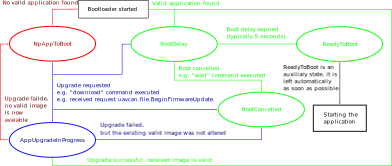
\includegraphics[width=1.1\textwidth]{bootloader_state_machine}}
	\caption{Bootloader state machine.\label{bootloader_state_machine}}
\end{figure}

\begin{ZubaxSimpleTable}{Bootloader states}{|c | l | X|}
State ID & State name & Comment \\
0 & NoAppToBoot & There is no valid application to boot; the bootloader will be waiting for commands forever.\\
1 & BootDelay & The bootloader will start the application in a few seconds, unless the boot is cancelled or a firmware update is requested.\\
2 & BootCancelled & There is a valid application to boot, however, boot was cancelled by an external command.\\
3 & AppUpgradeinProgress & Application is currently being upgraded. If interrupted, the bootloader will go into either \textbf{NoAppToBoot} or \textbf{BootCancelled}.\\
4 & ReadyToBoot & The application is about to boot. This state is very transient and is left automatically as soon as possible.
\end{ZubaxSimpleTable}
\clearpage
On Zubax GNSS 2, the boot delay is set to 5 seconds.
The bootloader supports the following communication interfaces:

\begin{ZubaxSimpleTable}{Bootloader communication interfaces}{| l | l | X | X |}
Intreface & Parameters & Protocol & Note\\
USB & CDC ACM & YMODEM, XMODEM, XMODEM-1K (autodetect) & When connected, the DCD port is inactive\\
DCD port (UART) & 115200-8N1(fixed) & Same as USB CDC ACM & Available only while USB is disconnected\\
CAN1 bus & Autoconfigured & UAVCAN firmware update protocol & Always available on CAN1. CAN2 is not used in the bootloader.
\end{ZubaxSimpleTable}

As can be seen from the table, there are two families of protocols: serial and CAN based; both are reviewed below.

\section{Error codes}

The table below provides definitions for the well defined error codes that can be reported by the bootloader.

\begin{ZubaxSimpleTable}{Error codes}{| l | X |}
0 & Success.\\
1 & Unknown error.\\
9001 & Application ROM driver error: erase failed.\\
9002 & Application ROM driver error: write failed.\\
10001 & The current state of the bootloader does not permit the requested operation.\\
10002 & Application image is too large for the device. Download has been aborted.\\
10003 & Failed to write the next downloaded chunk of the application image into the ROM.\\
20001 & X/YMODEM interface write has timed out.\\
20002 & X/YMODEM retries exhausted.\\
20003 & X/YMODEM protocol error.\\
20004 & X/YMODEM transfer has been cancelled by the remote.\\
20005 & X/YMODEM remote has refused to provide the file.\\
30001 & UAVCAN service request has timed out.\\
30002 & UAVCAN file downloading has been interrupted.\\
32767 & Unknown error.
\end{ZubaxSimpleTable}
\clearpage

\section{LED indication}

While the bootloader is running, the LED indicators behave as follows:
\begin{itemize}
\item The status LED is always on, which is the main indicator that the bootloader, rather than the firmware, is currently running
\item The CAN1 LED behaves normally as a CAN bus activity and load indicator, blinking once for 25 milliseconds every time the CAN1 controller successfully transmits or receives a CAN frame.
\item The CAN2 LED displays one of the blinking patterns shown below, depending on which state the bootloader is in. While the bootloader is running, the state of this LED has no relation to the state of the redundant CAN interface (which is CAN2), since the bootloader makes no use of it.
\end{itemize}

\begin{ZubaxSimpleTable}{LED patterns during bootloader stage}{| l | X |}
Bootloader state & LED blinking pattern (step 50 ms) \\
NoAppToBoot  & 10 Hz (very quickly)\\
BootDelay, ReadyToBoot  & Turned off\\
BootCancelled &  1 Hz, short pulses (50 ms)\\
AppUpgradeInProgress & 1 Hz, long pulses (500 ms)
\end{ZubaxSimpleTable}

\section{Via USB/UART}

Once started, the bootloader exposes a CLI via either DCD port or USB. The USB is always preferred if it is connected to the host; otherwise the CLI falls back to the UART interface of the DCD port.

The CLI can be used to query the state of the bootloader, modify it, obtain the information about the running firmware, and upgrade it if necessary.

The CLI prompt is of the following format: \textbf{StateName>}, which features the human readable name of the current state of the bootloader, followed by the ASCII greater character (ASCII code 62), followed by a space. For example:  \textbf{BootDelay>}. Such prompt allows the user (or software) to easily identify the state of the bootloader.

\subsection{CLI commands}

\textbf{reboot}

Restarts the bootloader.

\textbf{zubax{\_}id}

This is the standard command supported by all products by Zubax Robotics that have a CLI. It takes no arguments, and outputs a YAML key-value dictionary containing the vital information about the device, the firmware it is running, unique ID, installed certificates of authenticity, version of the hardware, and possibly some other information. Aside from the standard fields, this command also provides at least the following fields in its output:

\begin{itemize}
\item \textbf{bl{\_}version} - bootloader version, major and minor.
\item \textbf{bl{\_}vcs{\_}commit} - build identifier of the bootloader.
\item \textbf{mode} - set to the string \textbf{bootloader} to indicate that the bootloader is running.
\end{itemize}

If there is a valid firmware, its version information will also be provided via the standard fields \textbf{fw{\_}version} and  \textbf{fw{\_}vcs{\_}commit}. If the bootloader could not find a valid firmware, these fields will be omitted.

\textbf{wait}

Do not boot the application. If the current state is \textbf{BootDelay}, the state will be switched to \textbf{BootCancelled}. In all other states the command will have no effect.

\textbf{download}

Start the serial receiver and prepare to receive the new firmware image as a flat binary via the serial link using either YMODEM, XMODEM, or XMODEM-1K. The bootloader will automatically detect which protocol to use. According to the YMODEM specification, if no transfer was initiated by the host within one minute, the command will exit with an error. Possible error codes are defined in the table above.

Note that while this command is running, the CLI will be unavailable, since the same serial link will be temporarily occupied by the file transfer protocol.

If the YMODEM protocol is used, the file name field in the transfer header packet will be ignored.

There are heaps of software products and scripts that support these file transfer protocols. For instance, the popular program \textbf{sz} (available on most Linux distributions) can be used as follows:
\begin{minted}[linenos = false]{bash}
sz -vv --ymodem --1k \$file > \$port < \$port
\end{minted}

\section{Via CAN bus}

The bootloader supports the UAVCAN firmware update protocol. Please refer to the UAVCAN specification for theory.

The bootloader only utilizes the primary CAN interface, which is CAN1. The redundant interface CAN2 remains in the passive mode while the bootloader is running. It is therefore required that if there is only one interface in use, it must be CAN1.

The following table describes the mapping from the bootloader states to the UAVCAN node status codes:

\begin{ZubaxSimpleTable}{Bootloader states and UAVCAN node status codes}{| X | X | X |}
Bootloader state & UAVCAN node mode & UAVCAN node health\\
NoAppToBoot & SOFTWARE{\_}UPDATE & ERROR\\
BootDelay, ReadyToBoot & MAINTENANCE & OK\\
BootCancelled & MAINTENANCE & WARNING\\
AppUpgradeInProgress & SOFTWARE{\_}UPDATE & OK
\end{ZubaxSimpleTable}

The vendor specific status code of the node status message contains the status code of the last attempt to upgrade the firmware. Please refer to the error code table provided above.
\clearpage

\subsection{Supported messages}
\begin{ZubaxSimpleTable}{Supported messages}{| l | l | l | l |}
Data type & Direction & Period & Transfer priority \\
\texttt{uavcan.protocol.NodeStatus} & Output & 1 Hz & 24(low) \\
\texttt{uavcan.protocol.debug.LogMessage} & Output & Aperiodic & 31(lowest) \\
\texttt{uavcan.protocol.dynamic{\_}node{\_}id.Allocation} & Input/Output & Aperiodic & 24 (low)
\end{ZubaxSimpleTable}

\begin{ZubaxSimpleTable}{Supported messages annotation}{| l | X |}
Data type & Note\\
\texttt{uavcan.protocol.NodeStatus} & Refer to the bootloader state mapping table.\\
\texttt{uavcan.protocol.debug.LogMessage} & Used to report the application upgrade progress and status in a human readable form.\\
\texttt{uavcan.protocol.dynamic{\_}node{\_}id.Allocation} & Used only during initialization, if the application did not provide a specific node ID to use.
\end{ZubaxSimpleTable}
\clearpage

\subsection{Supported services}

\begin{ZubaxSimpleTable}{Supported servers}{| l | X |}
Data type & Note\\
uavcan.protocol.GetNodeInfo & The nested structure  \textbf{uavcan.protocol.SoftwareVersion} is populated only if there is a valid application.\\
uavcan.protocol.RestartNode & Restarts the bootloader.\\
uavcan.protocol.file.BeginFirmwareUpdate & Initiates the firmware update process, unless it was initiated earlier before the application has rebooted into the bootloader.
\end{ZubaxSimpleTable}

\begin{ZubaxSimpleTable}{Supported clients}{| l | l | l | X |}
Data type & Response timeout & Transfer priority & Note \\
uavcan.protocol.file.Read & 1 second & 24(low) & Used to download the application image file from the specified file server.
\end{ZubaxSimpleTable}

The interval at which the file read requests are issued while downloading the application image is defined by the following formula (all units SI):

\begin{equation}
\text{last{\_}response{\_}latency} + 1 / (1 + \text{can{\_}bus{\_}bit{\_}rate} / 65536)
\end{equation}

This formula, combined with the low transfer priority, allows the bootloader to avoid congestion of the CAN bus while downloading the firmware image.

\chapter{Mechanical characteristics}\label{sec:mechanical}

The drawing below documents the basic mechanical characteristics of Zubax GNSS 2,
such as the placement of connectors and mounting holes.

\begin{figure}[!hbt]
    \center
	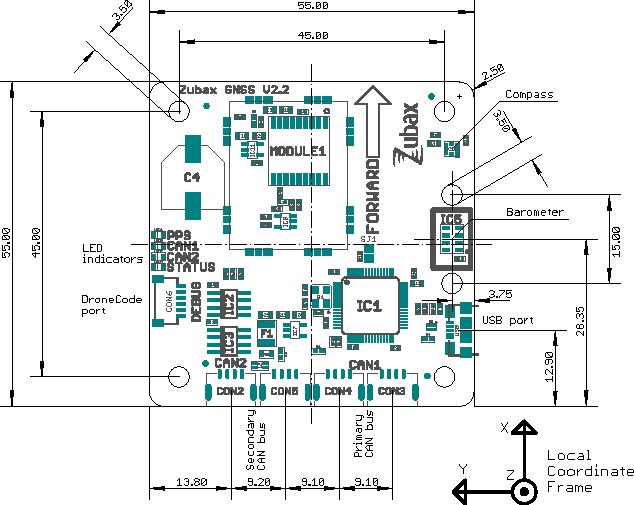
\includegraphics[width=1\textwidth]{GNSS2_drawing}
	\caption{GNSS2 drawing.\label{drawing}}
\end{figure}


\end{document}
